\documentclass[12pt]{report}
\usepackage[bindingoffset=0.2in,%
%			left=1in,right=1in,top=1.5in,bottom=1.5in,%
            left=2.45cm,right=2.45cm,top=4cm,bottom=4cm,%
			]{geometry}
\usepackage{graphicx}
\usepackage{fancyhdr}
\usepackage{setspace}
\fancyhf{}
\renewcommand{\headrulewidth}{0pt}
\fancyhead[RO,LE]{\thepage}
\pagestyle{fancy}
%\linespread{1.3}

\begin{document}
	
%	Page for Contents(Index)
	\tableofcontents
	\newpage
	
	
	\onehalfspacing
	
%	Page no - 27
	\begin{itemize}
		\item Frontal face, neutral expression, spot light added at the person’s left side.
		\item Frontal face, “joker image” (arbitrary expression), diffuse light.
	\end{itemize}
	\qquad The images are stored in 640 × 480 JPEG files. Owing to technique problems, most
	images are RGB, but some are grey-scale [66]. One good thing about this database is that
	manually labeled face contour is available. The following facial structures were annotated
	using 58 landmarks: eyebrows, eyes, nose, mouth and jaw. These landmarks are divided
	into seven point paths; three closed and four open as shown in Fig.2.14. In our work, this
	database will be used to train the ASM and AAM model.
	
	\begin{figure}[h]
		\centering
		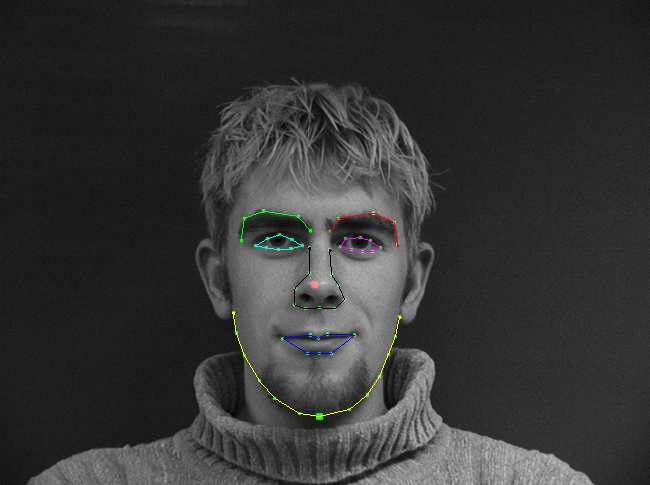
\includegraphics[scale=0.5]{img/fig_2-14.png}
		\caption{Example image from IMM face database}
	\end{figure}
	\vspace{0.5cm}
	\noindent \textbf{CMU Pose, Illumination, and Expression Database [79]} \vspace{0.3cm} \\
	The CMU-PIE database is among the most comprehensive databases in this area. It
	systematically samples a large number of pose and illumination conditions along with a
	variety of facial expressions. The PIE database was captured under 21 illuminations (lit by
	21 flashes) from 13 directions (using 13 synchronized cameras). In total, there are 41,368
	images obtained from 68 individuals. In our experiment, we only use a sub-set of this
	database which consists of images of 62 people. 25 images were selected for each individual
	
	
	
	\pagebreak
	
%	Page no - 28	
	\noindent with 5 different viewpoints and 5 different illuminations. Part of the data set is shown in
	Fig.2.15.
	
	\begin{figure}[h]
		\centering
		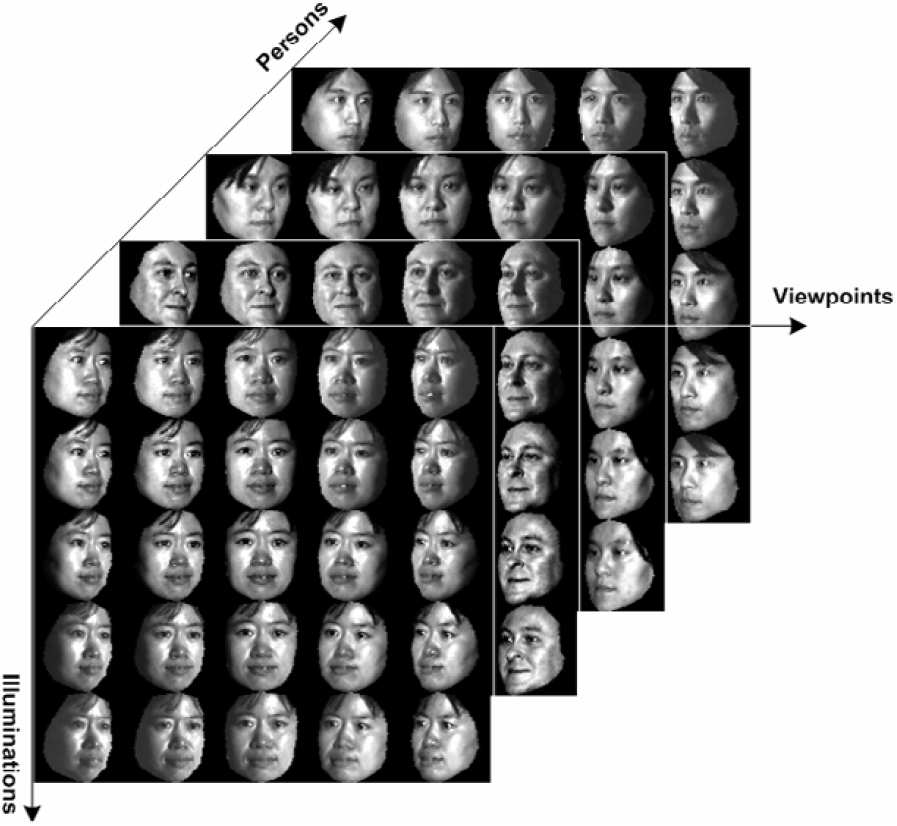
\includegraphics[scale=0.3]{img/fig_2-15.png}
		\caption{A subset of CMU PIE database [53]}
	\end{figure}
	\vspace{0.5cm}
	
	\noindent \textbf{\large 2.7.2 Databases for Expression Recognition} \vspace{0.3cm} \\
	``The human face is able to display an astonishing variety of expressions. Collecting a
	database that samples this space in a meaningful way is a difficult task'' [35]. As a result,
	there are many fewer databases available for expression recognition (Table 6.1). As men-
	tioned in 2.1.1, there are two ways to describe facial expressions. Available databases can
	be categorized into two classes according to the description they used. In one group [38]
	expressions are coded in FACS, while in the other group [57] images are labeled by their
	prototypic emotional expressions.
	\vspace{0.1cm} \\
	
	\noindent \textbf{Japanese Female Facial Expression Database [57]}
	\vspace{0.3cm} \\
	The JAFFE database contains 213 images of 10 Japanese female models. Their images are
	labeled by emotions: six basic emotions (anger, disgust, fear, joy, happy, sad and surprise)
	are considered and “Neutral” is added as the 7th emotion which is defined through the
	absence of expression. Fig.2.16 shows example images for one subject along with emotion
	
\end{document}
